\chapter{实验与结果分析}

\section{引言}

在本章,我们利用倾向值匹配算法对获取的数据进行实验分析,针对电视剧演员的不同行为模式进行比较,从而选取推广效果最好的推广策略推荐给演员,以求达到最好的宣传效果。首先,我们针对三种推广模式的十种推广策略,并引入演员的粉丝量作为混淆变量进行分析。通过分析结果可以看出,在首播后的阶段内,在早上发布更多的原创微博能够获得更好的推广效果。但是考虑到推广周期这一推广模式存在的问题,以及混淆变量数量过少对分析结果造成的影响,我们又提出了改进模型,对新获取的数据进行了新的实验。在改进实验中,将所有数据根据话题演化模型分为平稳期和爆发期两组,对于每组内的所有微博分析其推广时间和互动模式这两个推广模式的推广效果,并引入演员性别、电视剧评分等更多的混淆变量加入到模型当中,使得分析结果更具有可信性。同时我们还对分析结果进行了模型显著性检验和平衡性检验,验证了倾向值匹配算法的适用性和准确性。

\section{演员社交推广行为的影响力模型}

本节利用倾向值匹配算法,对演员发布的推广微博的影响力进行了建模,对不同的微博推广策略进行了对比,分析了不同推广策略所带来的不同的推广效果。

\subsection{实验数据}

本节选取爱奇艺和腾讯视频两个视频网站中,首次播放时间在2013年1月1日到2015年3月1日期间的222部电视剧作为研究对象。抓取电视剧的基本信息,包括电视剧主演、播时间、视频点击量等。同时在微博上抓取电视剧及其主演的微博数据。电视剧的微博数据包括电视剧相关微博话题的话题名称、话题阅读量、话题讨论量等;电视剧主演的微博数据包括222部电视剧所涉及的886个主演的个人信息和所发微博。其中个人信息包括演员的id、昵称、关注数、粉丝数、微博总数、注册时间以及演员的关注关系链等。演员所发微博数据包括所有发布的微博数目、内容、时间,以及每条微博下面的点赞数、转发数、评论数等信息,共计1671764条微博,其中与我们选定电视剧相关的有30959条微博。

\subsection{推广策略及混淆变量}

为研究演员社交行为对电视剧的推广作用,将演员发布的推广微博作为研究对象,根据3.3.2节的介绍,我们对三类推广模式下的10项推广策略进行研究,定义每一项推广策略为策略$t$,其取值为$T$。在我们的研究中,$T = {0, 1}$,其中$T = 1$代表采用这项策略,$T = 0$代表不采用这项策略。

\begin{table}[!htbp]
\centering
\caption{推广策略分类}
\begin{tabular}{|c|c|c|c|} \hline
\multicolumn{2}{|c|}{推广模式}&T=1&T=0\\ \hline
\multirow{3}{*}{推广周期} & 筹备阶段&筹备阶段发布&非筹备阶段发布\\% \hline
&首播阶段&首播阶段发布&非首播阶段发布\\% \hline
&首播后阶段&首播之后发布&非首播之后发布\\ \hline
\multirow{3}{*}{推广时间} &早上&早上发布&非早上发布\\% \hline
&中午&中午发布&非中午发布\\% \hline
&晚上&晚上发布&非晚上发布\\ \hline
\multirow{3}{*}{互动模式} &主演互动&与主演互动&非与主演互动\\% \hline
&与官微互动&与官微互动&非与官微互动\\% \hline
&原创&原创非互动&非原创\\ 
&其他互动&其他互动&非其他互动\\ \hline
\end{tabular}
\end{table}

当对某一项推广策略进行分析时,将其他策略视为混淆因素,加入混淆变量集合$X$。另外对于不同演员来说,其知名度和受欢迎程度对于推广微博的影响力有着很大的影响,更加流行的演员发布的微博能够收获更多的回复和点赞。而每个演员在微博上的粉丝数,是从侧面衡量演员流行度的一个指标。因此,我们将发布微博的演员的粉丝数同样作为一个混淆变量加入到模型当中,去除演员的粉丝数对分析结果的影响。由于不同演员的粉丝数量差别较大,有的著名演员拥有数百万的粉丝,而对于一些名气稍小的演员仅仅拥有几百或几千粉丝,因此为压缩粉丝数数据尺度,对各个演员的粉丝数取值为10的对数。

\subsection{算法应用}

根据第四章所介绍的方法,应用倾向值匹配算法对这些微博数据进行分析。

首先,对于要分析的每一项推广策略,可以将其他的推广策略视为混淆变量。那么对于全部待研究的十项推广策略来说,选取其中一项为研究对象,另外九项既为混淆变量,同时将演员的粉丝量也作为混淆变量,将其纳入逻辑斯地回归模型来计算每一条微博的倾向值。

然后,根据是否采用了这项策略,将所有计算出倾向值的微博分为两个样本集合,对两个样本集合中的微博根据其倾向值采用一对多匹配和基于卡尺的最近邻方法进行匹配。在基于卡尺的最近邻匹配过程中,经过对于实验数据的观察和分析,设置卡尺距离为0.09。

最后,计算平均干预效果ATT来衡量该项策略对结果的影响效果。用t-test来检验干预效果的显著性水平,即检验两组微博中的微博影响力水平是否有显著差异。

\subsection{结果分析}

通过倾向值匹配算法,得到针对不同推广策略的推广效果,可以更好地指导演员在社交网络上选择推广行为模式,提高电视剧收视热度。

\textbf{(1) 推广周期。}

按推广周期计算筹备阶段、首播阶段和首播后阶段的平均干预效果ATT如表~\ref{r1}所示。可以看到,在筹备阶段发布的微博的平均干预效果为负值,且t检验结果显著,说明筹备阶段发布的推广微博影响力不如非筹备阶段,即首播阶段和首播后阶段。而首播阶段发布微博的影响力效果虽然为负值,但是经过t检验,与非首播阶段发布微博的影响力效果没有显著差异。与二者相比,首播后阶段发布微博的影响力效果与筹备阶段和首播阶段相比有显著差异,会显著提高。分析原因可能是粉丝们在筹备阶段和首播阶段只能看到关于电视剧的少量信息和花絮,参与感较低,导致关注度不高;而当用户看过电视剧后,在演员利用微博进行电视剧推广时,粉丝们可以针对剧情、人物等积极参与讨论,对微博内容也可以有更多的态度和观点,此时进行推广,效果会更好。

\begin{table}[h]
\centering
\caption{推广周期策略比较}
\label{r1}
\begin{tabular}{|c|c|c|c|} \hline
推广周期 & ATT & 显著性\\ \hline
筹备阶段 & -674.204& 0.000\\ \hline
首播阶段 & -182.854& 0.260\\ \hline
首播后阶段 & 757.065 & 0.000\\ 
\hline\end{tabular}

\end{table}

\textbf{(2) 推广时间。}

计算各个推广时间干预效果ATT和t检验的结果如表~\ref{r2}所示。通过结果可以看出,三种推广时间策略都具有较高的显著性,但在早上发布微博的平均干预效果为正值,而其他两种策略的平均干预效果为负值。这说明,与想象中不同的是,早晨发布推广微博获得的推广效果要显著好于中午和晚上发布。原因可能是,推广信息具有时效性,对当天来说,早晨发布的微博一天中被看到的时长和概率是最大的,到了第二天,消息的时效性大大降低,导致粉丝的参与度大大降低。因此建议演员更多的在早晨发布推广微博。

\begin{table}[h]
\centering
\caption{推广时间策略比较}
\label{r2}
\begin{tabular}{|c|c|c|c|} \hline
推广时间& ATT & 显著性\\ \hline
早上 & 879.083& 0.000\\ \hline
中午 & -138.270& 0.036\\ \hline
晚上 & -314.376 & 0.000\\ 
\hline\end{tabular}

\end{table}

\textbf{(3) 互动模式。}

按互动模式将演员推广行为分为与其他主演互动,与官微互动,原创非互动和其他互动四种方式。经过倾向值匹配算法,得到结果如表~\ref{r3}所示。可以看到演员与其他主演互动、与官微互动和发布原创微博时,平均干预效果都有所增加,都对推广有显著效果。因为主演和主演互动本身就在制造话题性,与官微互动,会转发一些电视剧情节、花絮及与演员相关的信息,信息量较大,会增加粉丝参与。而原创非互动模式与非原创相比,平均干预效果显著提高,推广效果提高的最大。分析演员的微博可知,原创微博更能表达演员的情感和对粉丝参与的情感呼吁,因而更能得到粉丝的支持和参与,推广效果也会更好。与之对比,转发其他视频网站、粉丝的微博等其他互动方式的推广效果明显不如另外三种互动方式,不管从携带信息量还是从演员情感角度看,其他互动方式的宣传效果都会较差。

\begin{table}[h]
\centering
\caption{互动模式策略比较}
\label{r3}
\begin{tabular}{|c|c|c|c|} \hline
互动模式& ATT & 显著性\\ \hline
主演互动  & 759.315& 0.000\\ \hline
与官微互动 & 3413.222& 0.000\\ \hline
原创  & 12007.880& 0.000\\ \hline
其他互动 & -7195.497 & 0.000\\ 
\hline\end{tabular}
\end{table}

通过以上的实验结果可以看出,不同的推广策略能够带来不同的推广效果,利用倾向值匹配算分能够有效区分混淆变量对于因果分析的影响。但是在本节所介绍的实验中,我们仅仅将演员的粉丝量加入到混淆变量当中,即区分了演员不同的流行程度、人气指数对结果的影响。但是还有其他的众多因素能够影响推广效果,例如演员的性别、年龄、电视剧的演员阵容等,因此需要将更多的因素列入到混淆变量当中进行分析。同时,对于推广周期这一推广模式而言,由于大多数演员会在整个电视剧的宣传周期内持续发布众多的微博,虽然根据倾向值匹配的分析结果,在不同阶段发布的微博能够获得不同的推广效果,但这并不会影响演员发布推广微博的频率。而且通过对不同阶段发布的微博的分析可以发现,不同微博之间的内容、受关注程度等都存在较大差异,仅仅将其划分到不同的推广周期并不能清晰地体现出其中存在的差异。因此,并不应该将微博的推广周期视为一个较为合理的推广模式进行讨论。针对本节实验存在问题,我们提出了一种基于话题演化模型的改进方法,更好地对不同的推广模式进行了比较。

\section{基于话题演化的模型改进}

本节是对上一节应用的改进优化,使倾向值模型更合理的应用在演员推广行为的分析中。不但结合话题演化规律,将话题根据电视剧上映时间分成平稳期和爆发期,分别在两个时期分析演员的推广行为和推广策略,而且将更多会影响电视剧话题热度的因素考虑在内,使分析结果更具有可靠性。

\subsection{电视剧话题演化规律}

研究发现,微博热点话题在传播过程中,不仅关键词高度集中、受外界环境影响显著,而且传播具有周期性。话题周期一般包括话题发生、话题发展、话题高潮和话题消退四个阶段 \cite{赵龙文2013基于意见领袖参与行为的微博话题热度预测研究}。统计发现,电视剧微博话题演化符合话题演化的基本特征,具有一定的周期特性,如图~\ref{ning}所示,电视剧《柠檬初上》的话题发展正是经历了话题发生、话题发展、话题高潮和话题消退的过程。

在话题演化发展的过程中,“意见领袖”起到了重要的引导作用,他们在信息传播的网络中扮演了关键节点的角色,他们可以为其他人提供信息、传播态度,同时也起到了过滤作用,将其希望传播的信息传递给其他人,而将其不希望传播的信息截留在自身节点处。同样,在电视剧话题演化的过程中,演员就充当了意见领袖的作用,他们不仅拥有很庞大的粉丝群体,还有很大的社交影响力。他们发布的微博信息往往能受到高度关注,在电视剧话题发展过程中,演员发挥了核心作用。在电视剧话题发展过程中有三个重要时间节点导致了电视剧话题向下一阶段的发展,分别是电视剧上映时间确定、首集播出时间、首轮播出结束。在电视剧上映时间确定之前,演员会不时发些电视剧相关信息包括电视剧拍摄进度、拍摄期间趣事、角色定妆照等信息的微博,提前宣传使电视剧话题在微博产生。当电视剧上映时间确定后,主演通常都会发微博宣传电视剧,推动话题发展和酝酿,吸引粉丝和普通用户注意上映时间,吸引第一批群众。当电视剧首轮播放第一集之后,演员发布微博来吸引观看用户参与电视剧剧情、角色相关的讨论,用户也因为看过电视剧,在微博上更愿意参与到话题讨论中去,带来话题热度的大发展。演员和用户的这种行为会持续到电视剧首轮播放结束后几天,之后话题因为其时效性,最终走向消退。

\begin{figure}[!htbp]
\centering
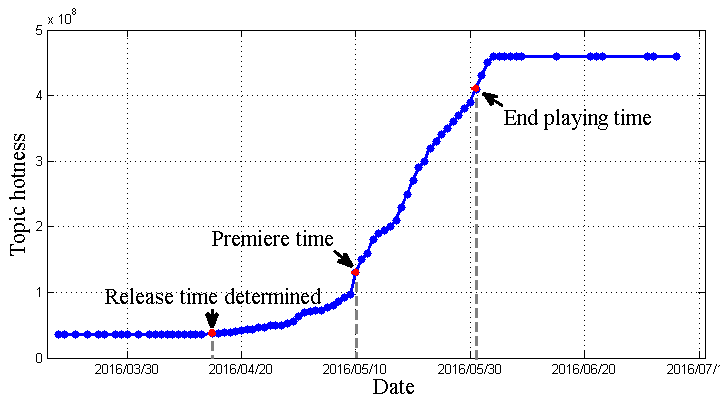
\includegraphics[width=9cm]{2}
\caption{电视剧《柠檬初上》的话题演化过程}
\label{ning}
\end{figure}

电视剧话题出现和发展期相对于话题爆发和消退期存在本质上的差别,即电视剧是否已经上映,带来用户对电视剧的内容了解的差异和参与方式的不同,进而导致话题热度发展不同。因此,本文中将电视剧话题根据电视剧是否上映分成两个主要时期,上映前为平稳期,上映后为爆发期。在电视剧话题的整个发展过程中,因为电视剧所处宣传期不同,演员在微博上不同时期的推广方式也会有差异。例如,对发布推广微博的时间,如图~\ref{time},在平稳期夜晚发布微博很少,白天不同时间发布微博数量比较平稳。但是在爆发期,在电视剧上映前后演员会有一个发布微博的高峰。在此时间发布微博不但能维持既有用户群观看电视剧、参与到电视剧话题讨论,还能吸引和号召新用户观看当天剧情。在不同时期演员发布推广微博的互动模式也有差异,从图~\ref{inter3}可以看出,与平稳期相比,爆发期演员会更多的与官方微博互动。因为当电视剧上映后,官方微博会发布更多的微博,包括剧情讨论、角色讨论、剧照、下集预告等等。

因此,研究演员在不同时期推广策略的有效性是非常有必要的。在本节,我们将演员发布的所有推广微博以电视剧上映的那一天作为时间节点,划分为两个时期分别进行讨论,即话题平稳期和话题爆发期。在各个时期内,利用倾向值匹配算法分析各个推广策略的推广效果。

\subsection{实验数据}

在本节,为了验证改进模型的可行性和准确性,我们又抓取了新的实验数据。通过爱奇艺爬虫,我们获取了2016年1月1日至2016年12月31日之间上映的所有电视剧和这些电视剧的所有主要演员姓名,一共有313部新的电视剧和1121位演员。根据这个电视剧名单,我们通过爱奇艺和豆瓣网站获取了这些电视剧的首播时间、观看量等数据。同时,在微博上获取了这些电视剧的话题数据、官方微博数据、主演数据。其中话题数据包括每天话题的讨论数和阅读数。官微和演员微博数据包括他们的基本信息和发布的所以微博信息,一共提取到了114767条微博。具体数据如表~\ref{data1}所示。

\begin{table}[!htbp]
\centering
\caption{实验数据}
\label{data1}
\begin{tabular}{|c|c|c|} \hline
数据集 & 数据名称 & 具体内容\\ \hline
\multirow{2}{*}{电视剧数据} & 豆瓣 & 豆瓣评分\\% \hline
& 爱奇艺 & 主演,首播时间,观看数\\ \hline
\multirow{3}{*}{微博数据} & 微博话题 & 讨论量,阅读量\\% \hline
& 官方账号 & 基本信息,微博\\% \hline
& 主演账号 & 基本信息,微博\\ \hline
\end{tabular}
\end{table}


\subsection{推广策略及混淆变量}

与上一小节相似,我们讨论推广时间和互动模式两个推广模式下的七种推广策略。而推广周期这一模式根据话题演化规律被分为平稳期和爆发期分别进行讨论,对分别属于这两个周期的所有微博进行倾向值匹配比较。

在倾向值匹配算法中,应该控制混淆变量使得混淆变量在策略组和非策略组分布相似,这样才能更好的分析策略的效果。考虑到影响一条微博在微博中热度的因素有很多,除了演员的推广策略本身,还受演员本身属性及电视剧属性等的影响,因此,本章中我们选用如表~\ref{mul}中包括演员和电视剧相关属性的信息作为混淆变量,使分析结果更具有可靠性。

\begin{table}[!htbp]
\centering
\caption{混淆变量}
\label{mul}
\begin{tabular}{|c|c|} \hline
种类 & 特征\\ \hline
\multirow{3}{*}{演员} & 粉丝数量\\% \hline
& 性别\\% \hline
& 作品数量\\ \hline
\multirow{2}{*}{电视剧} & 演员阵容\\% \hline
&豆瓣评分 \\ \hline
\end{tabular}
\end{table}

同样,在研究某一项推广策略时,将其他待研究的策略归为混淆变量,与以上介绍的这些混淆变量一起加入到混淆变量集合当中进行分析讨论。

\subsection{算法应用}

对于本实验来说,将倾向值匹配算法应用到实验数据上的方法与上一小节所介绍的实验类似。但由于采用了基于话题演化的模型改进,因此在开始进行分析之前,需要首先将所有微博根据发布的时间,以电视剧的首播时间为分割点,分为平稳期发布的微博和爆发期发布的微博两组,分别进行分析。

同时由于在本实验中,我们在社交网络上提取了更多的信息,也就可以在倾向值匹配模型中加入更多的混淆变量以更好地分析推广策略与推广效果之间的因果关系。而将这些混淆变量纳入逻辑斯地回归模型来计算每一条微博的倾向值的方法与上一节所介绍的方法相同。

然后,根据第3章所介绍的方法对已经得到倾向值的各个微博进行匹配,并对匹配结果计算平均干预效果来衡量该项策略对结果的影响效果。

\subsection{结果分析}

将倾向值匹配算法分别应用在演员推广的平稳期和爆发期,对各项推广策略进行因果分析,得到的推广策略有效性和t检验结果如表~\ref{res1}所示:

\begin{table}[!htbp]
\centering
\caption{基于话题演化模型的倾向值匹配结果}
\label{res1}
\begin{tabular}{|c|c|c|c|c|c|} \hline
\multicolumn{3}{|c|}{平稳期}& \multicolumn{3}{c|}{爆发期}\\ \hline
推广策略 & ATT & 显著性& 推广策略 & ATT & 显著性\\ \hline
早上 & -0.141 & 0.267& 早上 & 0.222 & 0.410\\% \hline
中午 & 0.023 & 0.837 & 中午 & 0.211 & 0.008\\% \hline
晚上 & 0.359 & 0.024 & 晚上 & -0.176 & 0.004\\ \hline
主演互动 & -0.088 & 0.561 &  主演互动 & -0.078 & 0.302\\
与官微互动& -0.318 & 0.002 & 与官微互动 & -0.001 & 0.989\\% \hline
原创& 2.633 & 0.000 & 原创& 1.860 & 0.000\\
其他互动& -0.743 & 0.000 & 其他互动 & -0.616 & 0.000\\ \hline
\end{tabular}
\end{table}

\textbf{(1)平稳期推广策略效果分析}

从表中可以看出,与在早晨和中午发布微博相比,在晚上发布微博的效果更好。用户晚上通常会花较多的时间在社交网络上,对他们而言,晚上发布的推广微博有更大的概率被他们看到。对互动模式而言,发布原创微博带来的推广效果要明显远远好于其他互动模式。与之相反,与官微互动和与其他人互动带来的推广效果较差。因为这种微博不能很好的表达演员自己的情感和想法,而且此时电视剧并未上映,粉丝参与电视剧推广微博更多的是因为演员,而不是因为剧情,因此对能更好表达演员自己想法和情感的原创微博会带来更好的粉丝参与度。与此同时,与其他主演互动的模式没有明显好的推广效果。

\textbf{(2) 爆发期推广策略效果分析}

在爆发期,下午发布的推广微博会带来更好的推广效果。在爆发期,演员通常在晚上会集中发很多微博,导致平均每条微博的粉丝参与度相对不高。从互动模式来看,发原创微博仍然是最有效的推广策略,原创微博需要演员投入更多的精力编写,同时更好的表达了他的想法和对粉丝参与的期望。而与其他人互动仍然效果最差,与官方微博和其他主演互动的推广效果并不显著。因此可知,在爆发期,演员在下午发布原创微博能获得更好的宣传效果。

\subsection{模型显著性及平衡性检验}

模型显著性及平衡性检验的作用是评估倾向值匹配模型是否恰当的进行了应用,对于待验证的各个策略来说,验证模型显著性即为验证所有混淆变量标准差在策略组和非策略组的平均值是否有显著差异,平衡性检验即为作累计分布图和分位数-分位数图(qq图)来看混淆变量在策略组和非策略组是否分布一致。表~\ref{res3}显示了两个时期,对于各个时间策略下,混淆变量的标准偏差。平稳期的标准偏差值在0.001到0.073之间,爆发期的标准偏差值在0.002到0.037之间,表明了策略组和非策略组的匹配样本的平均值分布一致。

\begin{table}[!htbp]
\centering
\caption{推广时间模式下,各个混淆变量的标准偏差}
\label{res3}
\begin{tabular}{|c|c|c|c|c|c|c|} \hline
&\multicolumn{3}{c|}{平稳期}& \multicolumn{3}{c|}{爆发期}\\ \hline
&早上&中午& 晚上 &早上&中午& 晚上\\ \hline
主演互动&0.012&0.073& 0.058&0.028&0.027& 0.008\\ \hline
与官微互动&0.029&0.007& 0.001&0.007&0.011& 0.003 \\ \hline
原创&0.053&0.006& 0.034&0.008&0.003& 0.008\\ \hline
其他互动&0.019&0.009& 0.047&0.018&0.006& 0.006\\ \hline
作品数量&0.006&0.023& 0.007&0.006&0.013& 0.007\\ \hline
性别&0.012&0.003& 0.054&0.023&0.047& 0.010\\ \hline
粉丝数量&0.008&0.033& 0.003&0.005&0.037& 0.002\\ \hline
演员阵容&0.012&0.033& 0.032&0.002&0.023& 0.003\\ \hline
豆瓣评分&0.030&0.049& 0.043&0.002&0.034&0.018\\ \hline
\end{tabular}
\end{table}

图~\ref{res2}显示的是在两个时期内,根据是否采用原创微博这条策略,绘制演员粉丝量、作品数、电视剧评分、电视剧阵容的累计分布图和分位数-分位数图,来刻画采用策略组和非采用策略组的混淆变量的分布情况。从图中可以看出,平稳期和爆发期的策略组和非策略组的这几个连续混淆变量的分布都非常类似。因此,倾向值匹配算法在我们的数据中得到了适当的应用,结果准确。

\begin{figure}[h]
  \centering%
  \subcaptionbox{平稳期\\.}
    {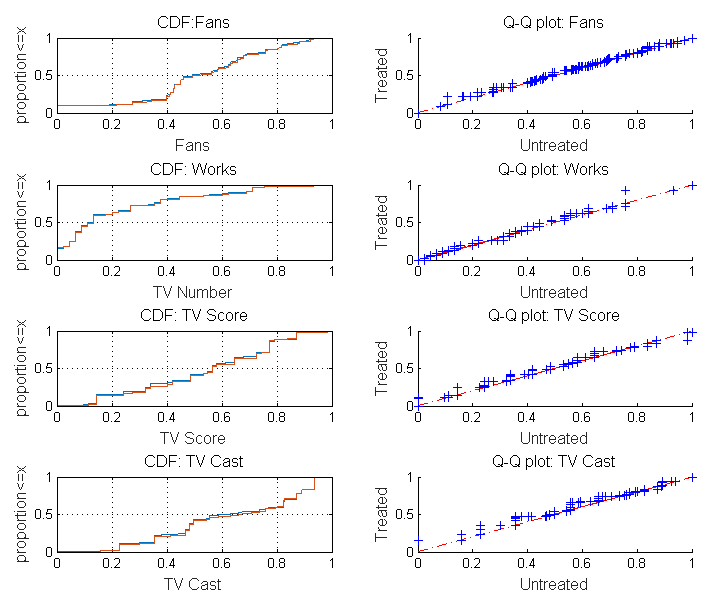
\includegraphics[width=12cm]{7}}
  \subcaptionbox{爆发期}
    {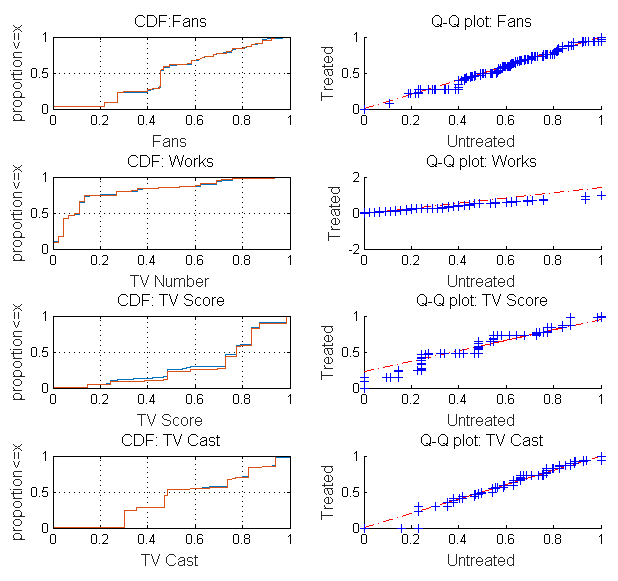
\includegraphics[width=12cm]{8}}
\caption{对于原创微博策略的平衡性检验}
\label{res2}
\end{figure}

\section{本章小结}

本章通过倾向值匹配算法对演员在微博上发布的推广微博进行了分析,针对不同演员不同电视剧的特点比较得出了最适合这个演员和这部电视剧的,具有最后推广效果的推广策略。在两组实验中,针对不同的演员和电视剧,通过倾向值匹配算法得到了不同的结论,比较得出了不同的最优推广策略,这充分验证的该算法对于不同比较对象所具有的针对性,利用该算法能够更有针对性地对演员的电视剧推广策略进行个性化的推荐,帮助其挑选出最优的推荐策略。



































